\documentclass[11pt,a4paper]{article}
\usepackage[margin=20mm,headheight=16pt]{geometry}
\usepackage{fontspec,kotex,amsmath,booktabs,longtable,array,xcolor,hyperref,fancyhdr,graphicx}
\setmainfont{DejaVu Serif}
\setsansfont{DejaVu Sans}
\setmonofont{DejaVu Sans Mono}
\setmainhangulfont{Noto Sans CJK KR}
\setmonohangulfont{Noto Sans CJK KR}
\definecolor{navy}{HTML}{173E59}
\definecolor{codebg}{HTML}{F3F6F8}
\hypersetup{colorlinks=true,linkcolor=navy,urlcolor=navy,pdftitle={GuardSynth Proposed Method}}
\urlstyle{same}
\setlength{\parindent}{0pt}
\setlength{\parskip}{6pt}
\setlength{\emergencystretch}{4em}
\setlength{\tabcolsep}{4pt}
\renewcommand{\arraystretch}{1.2}
\pagestyle{fancy}\fancyhf{}
\fancyhead[L]{\small GuardSynth}
\fancyhead[R]{\small Proposed Method}
\fancyfoot[C]{\thepage}
\renewcommand{\headrulewidth}{0.3pt}
\clubpenalty=10000\widowpenalty=10000
\raggedbottom
\begin{document}

\section*{IV. 제안 방법론}

\section*{A. 전체 접근과 입출력}

GuardSynth는 CoC에 담긴 행동 설명을 유지하면서, 행동 선택을 제한하는 조건을 별도의 명세로 명확하게 표현하고 다시 자연어로 결합하는 방법이다. 입력은 원래의 CoC, 판단에 사용할 장면 관측, 적용할 규칙과 그 근거이다. 출력은 구조화된 행동 제약, 제한된 모델에서의 논리 검증 결과, 명세에서 생성한 통제 자연어(CNL), 그리고 이를 원래 CoC에 추가한 학습 입력이다. 정형 표현은 조건의 의미와 검증 대상을 명시하고, 자연어 표현은 그 조건을 언어 기반 학습에 전달하는 역할을 한다.\par

전체 과정은 다음과 같다. 제약 후보의 선택과 근거 확인을 먼저 수행하고, 확정된 제약을 EBLC로 명세한다. 이후 구조와 의미를 검사하고 검증용 중간 표현을 거쳐 SMT 질의를 실행한다. 명세에 대응하는 CNL을 생성한 뒤, 원래 CoC와 결합하여 모델에 제공한다.\par

\par\medskip\noindent\begin{minipage}{\linewidth}\centering
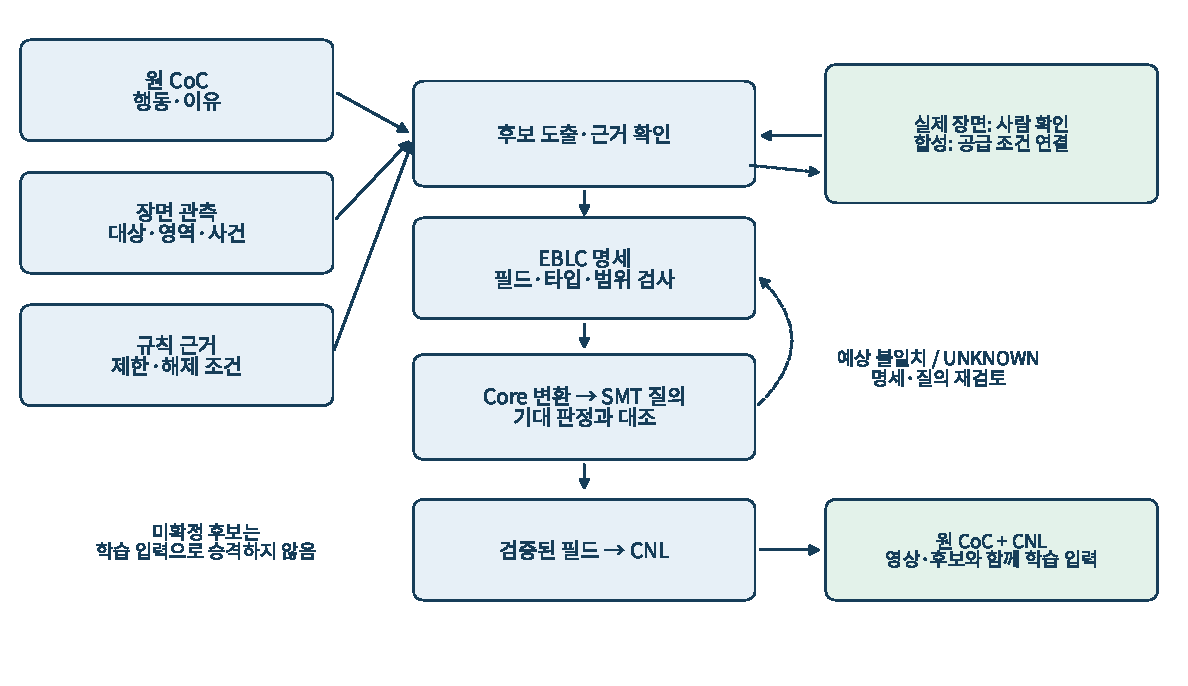
\includegraphics[width=\linewidth,height=.39\textheight,keepaspectratio]{figures/method-flow-ko.pdf}
\par\small\raggedright 그림 1. 실선은 정보의 전달 순서이고 점선은 미확정 근거나 예상과 다른 판정을 해당 단계로 돌려보내는 경로이다. 실제 장면의 사람 확인과 합성 실험의 공급 조건을 구분한다. 구조 검사 통과만으로 장면 적용이 승인되는 것은 아니다.
\end{minipage}\par\medskip

이 과정에서는 관측 사실, 규칙, 모델링 가정의 역할을 구분한다. 관측은 대상과 사건에 관한 정보를 제공하고, 규칙은 해당 상황에서 제한할 행동을 정한다. 가정은 검증 모델이 다루는 상황의 범위를 정한다. 예를 들어 영역이 비워지는 시점은 환경 정보이고, 비워진 뒤 대기해야 하는 기간은 규칙 정보이며, 이후 재점유가 없다는 조건은 모델링 가정이다. 동일한 관측에서도 적용 규칙이 다르면 허용 행동이 달라질 수 있다.\par

방법은 두 실행 프로파일로 구체화한다. 주 학습 실험에서는 공급된 합성 규칙을 수치 시간 계약으로 구성한다. 실제 장면을 다루는 별도의 정성적 프로파일에서는 관측과 사람 검토를 통해 대상·영역·사건을 연결한다. 두 프로파일은 명세와 근거를 연결한다는 원칙을 공유하지만, 입력과 의미론이 같지는 않다. 이하에서는 시간 계약을 일관된 주 예제로 사용하고, 정성적 프로파일은 근거 불확실성과 제약 수명주기를 설명하는 데 사용한다. 구현 근거는 \href{\detokenize{../../../../../../projects/04-guardsynth-coc/experiments/paper1_cnl_learning/temporal_preservation.py}}{S1}, \href{\detokenize{../../../../../../platforms/eblc-bcv/src/guard_synth_eblc/action_contract.py}}{S2}에 연결한다.\par

\section*{B. EBLC를 이용한 정형 명세}

\subsection*{1. 명세 범위와 구성 요소}

행동 제약은 특정 상황에서 선택 가능한 행동의 집합을 제한한다. 따라서 “무엇이 관찰되었는가” 또는 “왜 그 행동을 고려하는가”를 설명하는 문장과 구분된다. 또한 허용된 행동 중 무엇을 우선할지 정하는 목표와도 구별된다. 영역 진입을 허용하는 조건이 충족되었다고 해서 진입이 강제되는 것은 아니며, 허용 집합 안의 선택에는 별도의 목표가 필요하다.\par

Evidence-Bound Lifecycle Contracts(EBLC)는 이러한 제약을 적용 대상, 조건, 행동 제한, 유지와 해제, 근거와 함께 표현한다. Evidence-Bound는 명세의 조건과 규칙이 어떤 입력에 의존하는지 연결한다는 뜻이고, Lifecycle은 제약의 적용·유지·해제와 필요한 경우 재적용을 명시한다는 뜻이다. 이 논문은 그 구성 원칙과 구현된 제한 프로파일을 사용하며, 모든 교통 상황을 포괄하는 언어 정의를 전제하지 않는다.\par

\par\medskip\noindent\begin{minipage}{\linewidth}\small
\begin{tabular}{@{}>{\raggedright\arraybackslash}p{\dimexpr 0.2500\linewidth-4.000pt\relax}>{\raggedright\arraybackslash}p{\dimexpr 0.3300\linewidth-5.280pt\relax}>{\raggedright\arraybackslash}p{\dimexpr 0.4200\linewidth-6.720pt\relax}@{}}
\toprule
\textbf{구성 요소} & \textbf{명세에서의 역할} & \textbf{시간 계약의 구체화} \\
\midrule
주체와 대상 & 누구의 어떤 행동을 제한하는가 & 에고와 보행자 충돌 영역 \\
적용 범위 & 어느 상황·모델에서 해석하는가 & 단일 점유 해소, 이후 재점유 없음 \\
행동 제한 & 무엇을 허용하지 않는가 & 해제 조건 전의 영역 진입 \\
유지·해제 조건 & 언제 제한을 유지하거나 해제하는가 & 영역 해소 후 지정 기간 경과 \\
시간과 단위 & 시점·기간·경계를 어떻게 표현하는가 & 정수 밀리초, 경계값 포함 \\
근거와 버전 & 규칙의 출처와 해석 방식을 어떻게 식별하는가 & 규칙 참조와 프로파일 버전 \\
\bottomrule\end{tabular}\end{minipage}\par\medskip

정성적 프로파일은 이 구성에 사건의 진릿값, 근거 유효성, 초기 적용 상태와 복수 의무의 결합 정책을 추가한다. 이들은 불확실한 장면 근거를 다루기 위한 요소이며, 주 시간 학습 실험에서 모두 평가한 요소는 아니다. 본문의 명세 범위와 실험에서 확인한 범위를 구별하여 기술한다.\par

\subsection*{2. 계약의 정의와 해석}

두 프로파일을 설명하기 위해 계약을 {\ttfamily\small C = (s, z, \ensuremath{\Sigma}, O, E, V)}로 표기한다. s는 행동 주체, z는 대상 또는 영역, \ensuremath{\Sigma}는 적용 범위와 모델링 가정, O는 제한 의무의 집합, E는 관측·규칙 근거의 연결, V는 해석 버전이다. 이는 본문의 의미 설명을 위한 공통 표기이며, 여섯 필드를 가진 새 JSON 형식이 아니다. 실제 직렬화는 아래 코드 박스 1의 제한 프로파일을 따른다.\par

의무 하나는 시작 조건, 유지·해제 규칙, 제한 행동과 필요한 초기 상태로 해석한다. 시간 프로파일에서는 단일 해소 시점과 대기기간으로 이를 압축한다. 정성적 프로파일에서는 판단 시점마다 근거와 이전 상태로 적용 상태를 갱신한다. 두 프로파일의 가정과 상태 변수를 임의로 혼합하지 않는다.\par

h\_t를 판단 시점 t까지 제공된 근거와 상태의 이력, a를 현재 행동 후보라고 하자. 계약의 의미는 그 이력에서 허용되는 후보의 집합 {\ttfamily\small A\_C(h\_t)}이다. 후보가 이 집합에 속하면 명시한 조건과 제한에 부합한다. 복수 의무는 각각의 허용 집합을 교집합으로 결합하므로 모든 적용 제한을 동시에 만족해야 한다. 정성적 프로파일은 현재 해소 근거를 요구하는 진입 정책도 추가한다. 따라서 이전 금지가 비활성이라는 사실과 현재 진입 허용은 구별된다.\par

허용 집합을 정한 뒤 별도의 목표로 후보를 선택한다. 진입 보류와 충분히 기다린 뒤의 진입이 모두 허용되어도 진행 목표는 둘을 다르게 평가한다. 이 분리는 “제약을 위반하지 않음”을 “가장 좋은 행동임”으로 해석하는 오류를 방지한다.\par

\subsection*{3. 시간 프로파일의 구문과 의미}

시간 프로파일은 JSON 형태의 구조화된 계약을 입력으로 받는다. 다음은 0.5초 대기 규칙에 대해 실제 생성기가 반환하는 명세이다. 근거 참조는 추적용 메타데이터이며 모델이 선택할 정답 행동을 포함하지 않는다.\par

\par\medskip\noindent\begin{minipage}{\linewidth}
\textbf{코드 박스 1. 실제 생성된 시간 계약 JSON}\par

입력은 공급 규칙의 대기기간 0.5초이고, 출력은 대상·해제 조건·가정을 포함하는 계약이다. 줄 번호는 박스 내부의 위치를 나타낸다.\par

\par\medskip\noindent\fcolorbox{navy}{codebg}{\begin{minipage}{\dimexpr\linewidth-2\fboxsep-2\fboxrule\relax}
{\small\bfseries 코드 박스 1}\par\smallskip
\noindent\makebox[1.8em][r]{\color{gray}\scriptsize 1}\hspace{.8em}\parbox[t]{\dimexpr\linewidth-2.8em\relax}{\raggedright\ttfamily\fontsize{8.2}{10.5}\selectfont \hspace*{0.0em}\{\strut}\par\vspace{1pt}
\noindent\makebox[1.8em][r]{\color{gray}\scriptsize 2}\hspace{.8em}\parbox[t]{\dimexpr\linewidth-2.8em\relax}{\raggedright\ttfamily\fontsize{8.2}{10.5}\selectfont \hspace*{1.0em}"version": "supplied-temporal-eblc-profile-v0.1",\strut}\par\vspace{1pt}
\noindent\makebox[1.8em][r]{\color{gray}\scriptsize 3}\hspace{.8em}\parbox[t]{\dimexpr\linewidth-2.8em\relax}{\raggedright\ttfamily\fontsize{8.2}{10.5}\selectfont \hspace*{1.0em}"subject": "ego",\strut}\par\vspace{1pt}
\noindent\makebox[1.8em][r]{\color{gray}\scriptsize 4}\hspace{.8em}\parbox[t]{\dimexpr\linewidth-2.8em\relax}{\raggedright\ttfamily\fontsize{8.2}{10.5}\selectfont \hspace*{1.0em}"target": "pedestrian\_conflict\_zone",\strut}\par\vspace{1pt}
\noindent\makebox[1.8em][r]{\color{gray}\scriptsize 5}\hspace{.8em}\parbox[t]{\dimexpr\linewidth-2.8em\relax}{\raggedright\ttfamily\fontsize{8.2}{10.5}\selectfont \hspace*{1.0em}"hold": "NO\_ENTRY\_WHILE\_OCCUPIED",\strut}\par\vspace{1pt}
\noindent\makebox[1.8em][r]{\color{gray}\scriptsize 6}\hspace{.8em}\parbox[t]{\dimexpr\linewidth-2.8em\relax}{\raggedright\ttfamily\fontsize{8.2}{10.5}\selectfont \hspace*{1.0em}"release\_clear\_ms": 500,\strut}\par\vspace{1pt}
\noindent\makebox[1.8em][r]{\color{gray}\scriptsize 7}\hspace{.8em}\parbox[t]{\dimexpr\linewidth-2.8em\relax}{\raggedright\ttfamily\fontsize{8.2}{10.5}\selectfont \hspace*{1.0em}"time\_unit": "ms",\strut}\par\vspace{1pt}
\noindent\makebox[1.8em][r]{\color{gray}\scriptsize 8}\hspace{.8em}\parbox[t]{\dimexpr\linewidth-2.8em\relax}{\raggedright\ttfamily\fontsize{8.2}{10.5}\selectfont \hspace*{1.0em}"source\_kind": "SUPPLIED\_SYNTHETIC\_RULE",\strut}\par\vspace{1pt}
\noindent\makebox[1.8em][r]{\color{gray}\scriptsize 9}\hspace{.8em}\parbox[t]{\dimexpr\linewidth-2.8em\relax}{\raggedright\ttfamily\fontsize{8.2}{10.5}\selectfont \hspace*{1.0em}"assumption": "SINGLE\_CLEAR\_TRANSITION\_NO\_REOCCUPATION",\strut}\par\vspace{1pt}
\noindent\makebox[1.8em][r]{\color{gray}\scriptsize 10}\hspace{.8em}\parbox[t]{\dimexpr\linewidth-2.8em\relax}{\raggedright\ttfamily\fontsize{8.2}{10.5}\selectfont \hspace*{1.0em}"source\_refs": [\strut}\par\vspace{1pt}
\noindent\makebox[1.8em][r]{\color{gray}\scriptsize 11}\hspace{.8em}\parbox[t]{\dimexpr\linewidth-2.8em\relax}{\raggedright\ttfamily\fontsize{8.2}{10.5}\selectfont \hspace*{2.0em}"Project01/temporal\_guard\_world.py::\_guard",\strut}\par\vspace{1pt}
\noindent\makebox[1.8em][r]{\color{gray}\scriptsize 12}\hspace{.8em}\parbox[t]{\dimexpr\linewidth-2.8em\relax}{\raggedright\ttfamily\fontsize{8.2}{10.5}\selectfont \hspace*{2.0em}"paper1-method-preservation-v0.1"\strut}\par\vspace{1pt}
\noindent\makebox[1.8em][r]{\color{gray}\scriptsize 13}\hspace{.8em}\parbox[t]{\dimexpr\linewidth-2.8em\relax}{\raggedright\ttfamily\fontsize{8.2}{10.5}\selectfont \hspace*{1.0em}]\strut}\par\vspace{1pt}
\noindent\makebox[1.8em][r]{\color{gray}\scriptsize 14}\hspace{.8em}\parbox[t]{\dimexpr\linewidth-2.8em\relax}{\raggedright\ttfamily\fontsize{8.2}{10.5}\selectfont \hspace*{0.0em}\}\strut}\par\vspace{1pt}
\end{minipage}}\par\medskip
\end{minipage}\par\medskip

{\ttfamily\small subject}와 {\ttfamily\small target}은 주체와 제한 영역을 지정한다. {\ttfamily\small hold}는 점유 중 진입 금지를 나타내고, {\ttfamily\small release\_clear\_ms}는 영역이 해소된 뒤 요구하는 대기 기간이다. {\ttfamily\small assumption}은 점유에서 비어 있는 상태로 한 번 전환한 뒤 재점유되지 않는다는 가정을 지정한다. 이 가정이 있기 때문에 지속적인 비점유 상태를 하나의 해소 시점과 경과 시간으로 표현할 수 있다.\par

코드 박스 1의 2–5행은 버전과 제한 대상을, 6–7행은 대기값과 단위를 지정한다. 8–9행은 공급된 합성 규칙이라는 출처 유형과 재점유 없음 가정이며, 10–13행은 근거 참조이다. 관측의 해소 시각과 후보 진입 시각은 규칙 JSON에 섞지 않고 별도로 연결한다.\par

계약을 평가할 때는 환경에서 얻은 {\ttfamily\small clear\_ms}, 후보의 {\ttfamily\small entry\_ms}, 진입 여부인 {\ttfamily\small enters}를 별도로 연결한다. 두 시간 변수는 정수 밀리초이고, {\ttfamily\small enters}는 진입하는 후보이면 참이다. 시간 계약의 행동 제한은 다음과 같다.\par

\[\mathit{enters}\ \Longrightarrow\ \mathit{entry\_ms}\geq\mathit{clear\_ms}+\mathit{release\_clear\_ms}.\]

예를 들어 {\ttfamily\small clear\_ms = 11000}, {\ttfamily\small release\_clear\_ms = 500}이면 진입 후보는 11500ms 이상에서만 계약과 양립한다. 경계의 비교 연산은 ‘이상’이므로 11500ms는 허용되고 11499ms는 허용되지 않는다. 진입하지 않는 후보는 {\ttfamily\small enters = false}로 표현하며 이 진입 제한을 위반하지 않는다. 해당 후보의 진행 성과는 별도로 평가한다.\par

현재 시간 프로파일 검증기는 지원된 버전과 고정 필드 조합을 검사하며, 지원 대기값은 500, 1500, 800, 1800ms이다. 주 확장 학습 데이터는 그중 500과 1500ms를 사용한다. 임의의 필드를 가진 JSON을 범용 계약으로 받아들이는 방식이 아니라, 해석이 정해진 제한 프로파일을 사용한다. \href{\detokenize{../../../../../../projects/04-guardsynth-coc/experiments/paper1_cnl_learning/temporal_preservation.py}}{S1}, \href{\detokenize{../../../../../../projects/04-guardsynth-coc/experiments/paper1_cnl_learning/temporal_training_data.py}}{S3}\par

같은 의미를 {\ttfamily\small \ensuremath{\tau} = clear\_ms}, {\ttfamily\small \ensuremath{\Delta} = release\_clear\_ms}, {\ttfamily\small u = entry\_ms}, {\ttfamily\small e = enters}로 축약하면 {\ttfamily\small P\_C(e,u,\ensuremath{\tau}) = (\ensuremath{\neg}e) \ensuremath{\lor} (u \ensuremath{\geq} \ensuremath{\tau} + \ensuremath{\Delta})}이다. P\_C가 참인 후보가 시간 계약의 허용 집합에 속한다. 진입 후보에서는 경과 시간 {\ttfamily\small u \ensuremath{-} \ensuremath{\tau} \ensuremath{\geq} \ensuremath{\Delta}}를 요구하고, 비진입 후보에서는 진입 시각에 무관하게 참이다. \ensuremath{\tau}와 u는 시점이고 \ensuremath{\Delta}는 기간이다. “영역이 비었다”와 “필요한 기간만큼 비어 있었다”를 구분하는 식이다.\par

\subsection*{4. 정성적 프로파일의 수명주기 의미}

실제 장면용 정성적 계약에서는 각 의무 j와 판단 시점 t에 대해 {\ttfamily\small truth[j,t]}, {\ttfamily\small valid[j,t]}, {\ttfamily\small active[j,t]}를 사용한다. {\ttfamily\small truth}는 제한 조건이 확인되었는지를 TRUE, FALSE, UNKNOWN, CONFLICT로 나타낸다. FALSE는 해당 조건의 해소가 확인되었다는 뜻이고, 관측되지 않았다는 이유만으로 부여하는 값이 아니다. {\ttfamily\small valid}는 해당 근거를 수용할 수 있는지를 나타낸다. {\ttfamily\small active}는 그 의무가 적용 중인지 나타내며, 첫 판단 전의 값은 별도 입력으로 받는다.\par

\par\medskip\noindent\begin{minipage}{\linewidth}
\textbf{코드 박스 2. 근거에 따른 상태 갱신 의사코드}\par

입력은 의무 j의 현재 근거 진릿값·유효성 및 이전 적용 상태이고, 출력은 현재 적용 상태이다. 실행 소스 발췌가 아니라 의미론을 요약한 의사코드이다.\par

\par\medskip\noindent\fcolorbox{navy}{codebg}{\begin{minipage}{\dimexpr\linewidth-2\fboxsep-2\fboxrule\relax}
{\small\bfseries 코드 박스 2}\par\smallskip
\noindent\makebox[1.8em][r]{\color{gray}\scriptsize 1}\hspace{.8em}\parbox[t]{\dimexpr\linewidth-2.8em\relax}{\raggedright\ttfamily\fontsize{8.2}{10.5}\selectfont \hspace*{0.0em}on[j,t] = valid[j,t] AND (truth[j,t] = TRUE)\strut}\par\vspace{1pt}
\noindent\makebox[1.8em][r]{\color{gray}\scriptsize 2}\hspace{.8em}\parbox[t]{\dimexpr\linewidth-2.8em\relax}{\raggedright\ttfamily\fontsize{8.2}{10.5}\selectfont \hspace*{0.0em}clear[j,t] = valid[j,t] AND (truth[j,t] = FALSE)\strut}\par\vspace{1pt}
\noindent\makebox[1.8em][r]{\color{gray}\scriptsize 3}\hspace{.8em}\parbox[t]{\dimexpr\linewidth-2.8em\relax}{\raggedright\ttfamily\fontsize{8.2}{10.5}\selectfont \hspace*{0.0em}active[j,t] = TRUE,             if on[j,t]\strut}\par\vspace{1pt}
\noindent\makebox[1.8em][r]{\color{gray}\scriptsize 4}\hspace{.8em}\parbox[t]{\dimexpr\linewidth-2.8em\relax}{\raggedright\ttfamily\fontsize{8.2}{10.5}\selectfont \hspace*{7.0em}FALSE,           else if clear[j,t]\strut}\par\vspace{1pt}
\noindent\makebox[1.8em][r]{\color{gray}\scriptsize 5}\hspace{.8em}\parbox[t]{\dimexpr\linewidth-2.8em\relax}{\raggedright\ttfamily\fontsize{8.2}{10.5}\selectfont \hspace*{7.0em}previous\_active, otherwise\strut}\par\vspace{1pt}
\end{minipage}}\par\medskip
\end{minipage}\par\medskip

각 시점의 근거를 읽고 적용 상태를 갱신한 후 행동을 제한한다. 유효한 시작 근거는 의무를 적용하고, 유효한 해소 근거는 해제한다. 어느 쪽도 확인되지 않으면 이전 상태를 유지한다. 해제 이후 시작 조건이 다시 확인되면 같은 규칙으로 재적용한다. 이 순서와 초기 상태를 명시하여 판단 시점의 차이로 의미가 바뀌지 않도록 한다.\par

현재 정책은 선언된 모든 의무의 해소가 확인되어야 영역 진입을 허용한다. 어떤 의무의 이전 {\ttfamily\small active}가 거짓이더라도 현재 해소를 확인하지 못했다면, 그 사실만으로 진입을 허용하지 않는다. 반대로 모든 의무가 해소되면 진입과 진입 보류를 모두 허용한다. 이는 허용 조건이며 반드시 진행한다는 생존성 보장은 아니다. UNKNOWN·CONFLICT는 이 계약의 근거 상태이고, SMT 솔버가 결론을 내리지 못했을 때의 UNKNOWN 반환과는 구별된다. \href{\detokenize{../../../../../../platforms/eblc-bcv/src/guard_synth_eblc/action_contract.py}}{S2}\par

코드 박스 2의 1–2행은 유효성과 진릿값을 함께 확인한다. 3–5행은 시작, 해소, 그 외의 순서로 상태를 정한다. 첫 판단의 {\ttfamily\small previous\_active}는 별도 입력 {\ttfamily\small prior\_active}이고, 이후에는 직전 판단의 적용 상태이다. 단일 진릿값은 TRUE와 FALSE일 수 없으므로 시작과 해소가 동시에 참인 경우는 발생하지 않는다.\par

\par\medskip\noindent\begin{minipage}{\linewidth}\centering
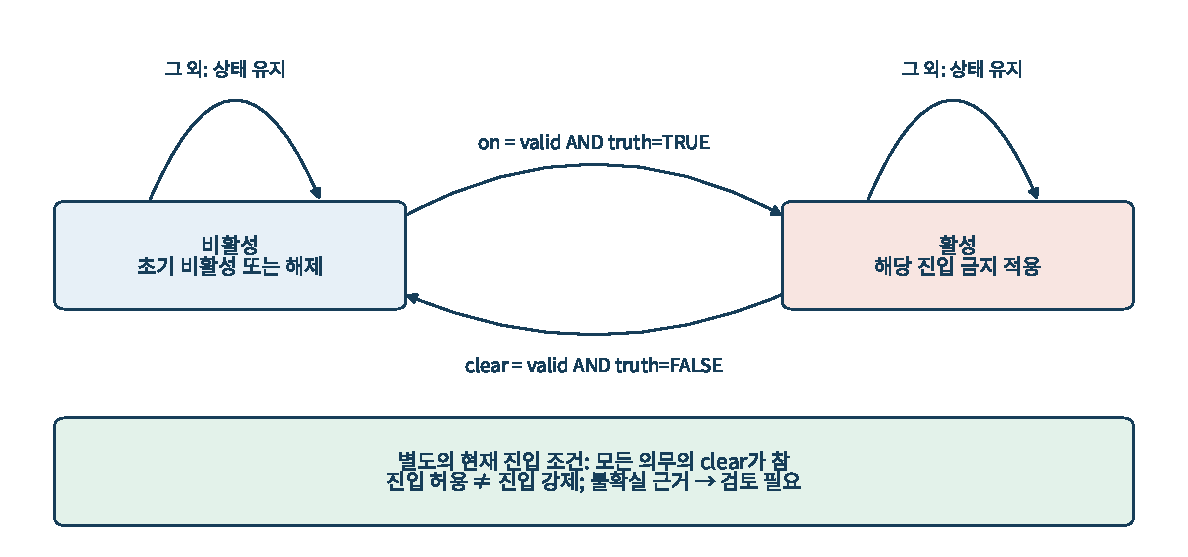
\includegraphics[width=\linewidth,height=.39\textheight,keepaspectratio]{figures/lifecycle-ko.pdf}
\par\small\raggedright 그림 2. 위쪽은 의무 하나의 상태 전이이고 아래쪽은 모든 의무를 결합한 현재 진입 허용 조건이다. 비활성에는 해제된 상태와 초기 비활성이 모두 포함된다. 비활성이라는 사실만으로 진입을 허용하는 연결은 두지 않는다.
\end{minipage}\par\medskip

현재 정책은 {\ttfamily\small entry\_permitted[t] = AND\_j clear[j,t]}이며, ENTER\_ZONE 행동은 이 값이 참일 때만 가능하다. DEFER\_ENTRY는 이 진입 금지를 위반하지 않는다. 불확실·충돌·무효 근거는 별도로 {\ttfamily\small review\_required}를 참으로 만든다. 예를 들어 초기 비활성인 의무 하나에 유효한 근거 TRUE \ensuremath{\rightarrow} UNKNOWN \ensuremath{\rightarrow} FALSE \ensuremath{\rightarrow} TRUE가 주어지면 상태는 활성 \ensuremath{\rightarrow} 활성 \ensuremath{\rightarrow} 비활성 \ensuremath{\rightarrow} 활성이다. 세 번째 판단에서만 진입이 허용되며, 그때도 보류를 선택할 수 있다. 이는 의미 설명을 위한 구성 예제이다.\par

\section*{C. 행동 제약의 정의와 추출}

\subsection*{1. 제약 후보와 근거의 분리}

CoC의 모든 문장을 제약으로 바꾸지는 않는다. “보행자가 횡단하고 있다”는 관측 주장이고, “보행자를 보호하기 위해 양보한다”는 행동 이유이다. “해당 영역이 점유된 동안 진입하지 않는다”는 조건과 행동 제한을 포함하므로 제약 후보가 된다. “허용된 후보 중 진행 성과가 가장 큰 것을 선택한다”는 제한 자체가 아니라 선택 목표이다. 이 구분을 통해 이유 설명에 없는 수치 임계값이나 해제 조건을 임의로 추가하는 일을 피한다.\par

입력 근거는 세 역할로 나눈다. CoC는 관련 행동과 의무의 후보를 찾는 데 사용한다. 장면 관측은 대상, 영역, 사건과 시점을 연결한다. 공급된 규칙 또는 별도로 확인한 규범 근거는 제한의 적용 조건과 내용을 정한다. 어떤 문장이 CoC에 존재한다는 사실만으로 그 문장의 현재 장면 적용까지 확인된 것으로 취급하지 않는다.\par

\subsection*{2. 명세화 절차와 자동화 범위}

먼저 CoC에서 행동과 관계된 대상·상황·판단 이유를 식별한다. 다음으로 대상과 영역을 관측에 연결하고, 어떤 시점의 사실인지 명시한다. 규칙 근거에서 제한 행동과 적용 조건을 정한 뒤, 유지·해제·시간 조건과 필요한 가정을 채운다. 확인하지 못한 정보는 추정 사실로 승격시키지 않고 미확정 상태로 남긴다. 확정한 내용은 지원 프로파일의 필드에 대응시키고, 근거 참조와 버전을 함께 기록한다.\par

주 합성 실험에서는 이 과정의 입력이 생성 환경과 공급 규칙에 의해 주어진다. 환경의 해소 시점과 규칙의 대기값을 읽어 계약을 구성하고 검증용 표현으로 변환한다. 따라서 이 경로의 자동화는 이미 주어진 조건의 구조화·변환이며, 영상만으로 법규나 대기시간을 발견하는 절차가 아니다. 실제 장면 경로는 사람이 대상·영역·사건과 적용 조건을 확인하며, 구현된 장면 adapter도 특정 검토 과제에 제한된다. \href{\detokenize{../../../../../../projects/04-guardsynth-coc/experiments/paper1_cnl_learning/temporal_training_data.py}}{S3}, \href{\detokenize{../../../../../../projects/04-guardsynth-coc/src/guard_synth/qualitative_scene_contract.py}}{S4}\par

추출 결과와 학습 정답은 별도로 관리한다. 제약에서 어떤 행동이 허용되는지를 정의하더라도, 실제 장면의 정답이 자동으로 확정되는 것은 아니다. 주 합성 과제에서는 알려진 환경 상태와 규칙을 이용한 별도의 정수 연산으로 허용 후보를 구하고, 그 안에서 진행 점수가 가장 큰 후보를 참조 행동으로 선택한다. 이 참조 계산은 CNL 문장이나 SMT의 판정값을 읽어 정답을 복제하지 않지만, 같은 환경·규칙 가정을 공유한다.\par

\par\medskip\noindent\begin{minipage}{\linewidth}\centering
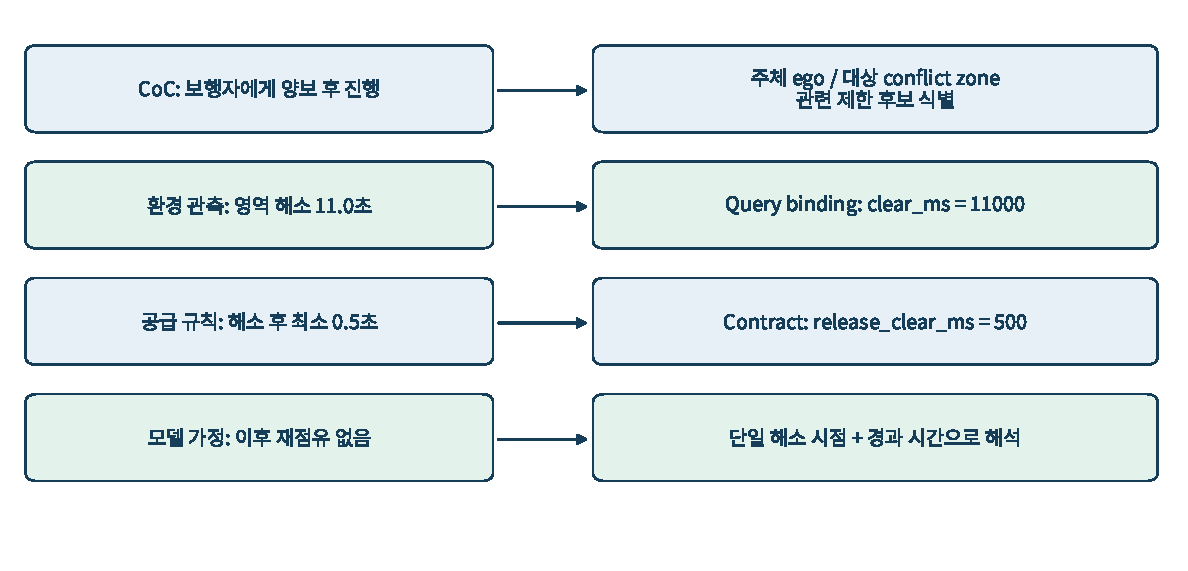
\includegraphics[width=\linewidth,height=.39\textheight,keepaspectratio]{figures/evidence-map-ko.pdf}
\par\small\raggedright 그림 3. 11.0초 해소 시점은 환경 관측으로서 질의 변수에 연결하고, 0.5초 대기는 공급 규칙으로서 계약 필드에 기록한다. 재점유 없음은 이를 시간 부등식으로 연결할 때의 가정이다. 제약 추출은 이러한 역할을 구분해 근거가 있는 필드를 구성하는 절차이다.
\end{minipage}\par\medskip

\subsection*{3. 이어지는 시간 예제}

주 예제의 원래 CoC는 “Yield to the crossing pedestrian, then proceed through the intersection.”이다. 환경은 영역이 11.0초에 비워진다고 제공하고, 별도의 공급 규칙은 최소 0.5초 또는 1.5초의 대기를 요구한다. 대기값은 CoC 문장에서 추론한 값이나 보편적 교통 법규가 아니라 명시적으로 공급된 실험 조건이다.\par

\par\medskip\noindent\begin{minipage}{\linewidth}\small
\begin{tabular}{@{}>{\raggedright\arraybackslash}p{\dimexpr 0.1500\linewidth-4.800pt\relax}>{\raggedright\arraybackslash}p{\dimexpr 0.1800\linewidth-5.760pt\relax}>{\raggedright\arraybackslash}p{\dimexpr 0.1900\linewidth-6.080pt\relax}>{\raggedright\arraybackslash}p{\dimexpr 0.2400\linewidth-7.680pt\relax}>{\raggedright\arraybackslash}p{\dimexpr 0.2400\linewidth-7.680pt\relax}@{}}
\toprule
\textbf{후보} & \textbf{진입 시점} & \textbf{진행 점수} & \textbf{0.5초 대기} & \textbf{1.5초 대기} \\
\midrule
A & 10.5초 & 110 & 위반 & 위반 \\
B & 11.5초 & 100 & 허용·참조 선택 & 위반 \\
C & 12.5초 & 85 & 허용 & 허용·참조 선택 \\
D & 진입하지 않음 & 0 & 허용 & 허용 \\
\bottomrule\end{tabular}\end{minipage}\par\medskip

진행 점수는 후보 선택을 위한 합성 효용이며 거리나 속도의 측정값이 아니다. 0.5초 계약에서는 B, 1.5초 계약에서는 C가 허용 후보 중 최대 점수를 갖는다. D는 두 계약을 위반하지 않지만 목표 진행을 완료하지 않는다. 이 표는 생성된 데이터의 한 구성이고, 모델이 실제로 이 답을 예측했다는 성능 사례가 아니다. 후보 라벨은 데이터 구성 과정에서 회전하여 고정된 문자만으로 답을 선택하지 않도록 한다.\par

\section*{D. CoC와 연결된 EBLC 명세의 검증}

\subsection*{1. 연결 확인과 Core 변환}

검증에는 의미를 정하는 입력 연결과 논리 질의 실행이 모두 필요하다. 주체와 대상 영역, 사건 시점, 규칙의 대기값이 같은 사례를 가리키는지 확인하고, 명세가 지원 버전·필드·단위를 만족하는지 검사한다. 근거 식별자는 입력을 추적하는 수단이며 사실의 진위를 스스로 증명하는 장치는 아니다. 실제 장면에서 연결되지 않은 필드는 조건부 명세와 구분해 관리하며, 구문 검사를 통과했다는 이유만으로 검토가 완료된 학습 자료로 취급하지 않는다.\par

시간 계약은 {\ttfamily\small enters}를 Boolean, {\ttfamily\small clear\_ms}와 {\ttfamily\small entry\_ms}를 정수로 선언하는 Core 표현으로 변환한다. {\ttfamily\small release\_clear\_ms}는 비교식의 정수 상수로 들어간다. Core는 검증에 필요한 선언과 논리 조항을 담는 중간 표현이며, 그 표현을 타입 검사한 뒤 SMT로 컴파일한다. 구현에서 시간은 밀리초 tick 수로 표현되고 Core의 단위 표기 {\ttfamily\small 1}을 사용한다. 이 표기를 초 단위 값으로 해석하지 않는다. 현재 계약의 변수는 시불변이고 조항은 초기 위치에 적용된다. Core의 {\ttfamily\small horizon = 2}는 이 구성의 모델 범위이지 2초 주행 궤적 검증을 뜻하지 않는다. \href{\detokenize{../../../../../../projects/04-guardsynth-coc/experiments/paper1_cnl_learning/temporal_preservation.py}}{S1}\par

\subsection*{2. 검증 속성과 질의}

\par\medskip\noindent\begin{minipage}{\linewidth}\centering
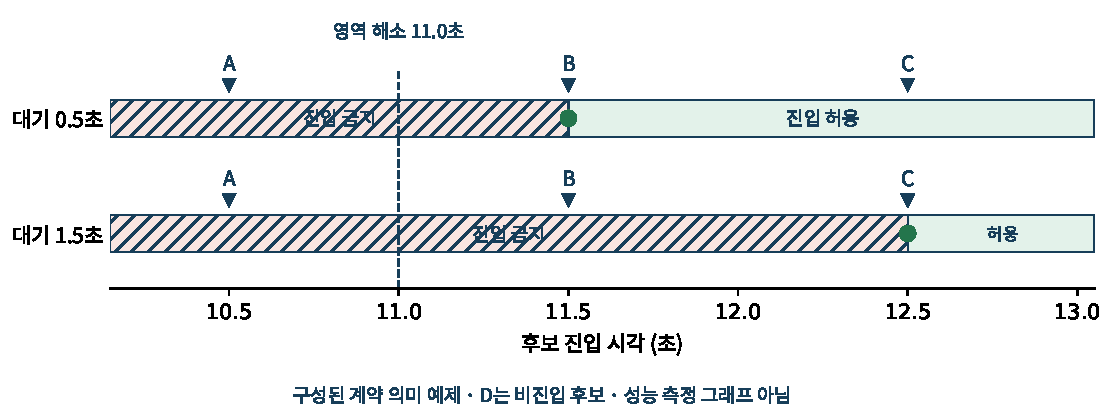
\includegraphics[width=\linewidth,height=.39\textheight,keepaspectratio]{figures/temporal-boundary-ko.pdf}
\par\small\raggedright 그림 4. 수평축은 초 단위 진입 시각이다. 해소 시점은 같지만 대기에 따라 허용 시작점은 11.5초 또는 12.5초가 된다. 닫힌 경계점은 그 시각 자체가 허용됨을 뜻한다. D는 비진입 후보이므로 시간축의 점으로 표시하지 않는다. 이 그래프는 계약 의미의 계산 결과이며 모델 정확도나 실측 주행 성능이 아니다.
\end{minipage}\par\medskip

검증은 일관성, 제한 조건, 해제 경계, 허용 가능성을 구분한다. 기본 명세의 SAT는 적어도 하나의 만족 모델이 있음을 확인한다. 그러나 진입하지 않는 경우만으로도 SAT일 수 있으므로, 해제 후 진입하는 만족 모델이 존재하는지도 별도로 확인한다. 허용 가능성의 확인은 모든 행동을 막는 명세를 피하기 위한 것이며, 모델의 실제 진행 성능을 대신하지 않는다.\par

\par\medskip\noindent\begin{minipage}{\linewidth}\small
\begin{tabular}{@{}>{\raggedright\arraybackslash}p{\dimexpr 0.2200\linewidth-5.280pt\relax}>{\raggedright\arraybackslash}p{\dimexpr 0.2000\linewidth-4.800pt\relax}>{\raggedright\arraybackslash}p{\dimexpr 0.3000\linewidth-7.200pt\relax}>{\raggedright\arraybackslash}p{\dimexpr 0.2800\linewidth-6.720pt\relax}@{}}
\toprule
\textbf{항목} & \textbf{질의 내용} & \textbf{기대 판정} & \textbf{해석} \\
\midrule
일관성 & 기본 계약 & SAT & 계약을 만족하는 경우가 존재 \\
제한 조건 & 진입하며 해제 시점보다 이르게 진입 & UNSAT & 제한을 위반하는 진입과 계약은 양립 불가 \\
경계 이전 & 11.499초 진입, 대기 0.5초 & UNSAT & 해제 직전 진입은 배제 \\
경계 시점 & 11.500초 진입, 대기 0.5초 & SAT & 경계값은 허용 \\
경계 이후 & 11.501초 진입, 대기 0.5초 & SAT & 해제 후 진입 가능한 경우 존재 \\
진입 보류 & enters가 거짓 & SAT & 진입을 강제하지 않음 \\
\bottomrule\end{tabular}\end{minipage}\par\medskip

시간값은 영역 해소 시점 11.0초를 기준으로 한다. 제한 조건 질의에서는 {\ttfamily\small enters}가 참이면서 {\ttfamily\small entry\_ms < clear\_ms + release\_clear\_ms}인 반례를 찾는다. 이 질의는 두 시간을 특정 값으로 고정하지 않는 상징적 질의이고, 나머지 경계 행은 구체적 값을 연결한 질의이다. 상징적 결과도 인코딩한 시간 부등식과 가정에 대한 결과이며, 영상의 해석이나 규칙 선택을 증명하지 않는다.\par

원고 예제의 여섯 질의를 500ms와 1500ms 계약에 각각 실행하여 12개 판정의 일치를 확인했다. 기존 bridge 검증의 100개 질의는 별도로 재실행했으며, 두 집합을 새로운 학습 효과의 근거로 합산하지 않는다. 검증 로그에는 질의, 기대 판정, 관측 판정과 실제 SMT-LIB 표현을 남겼다. \href{\detokenize{../methodology-2026-09-30-001/manuscript_examples.json}}{S5}\par

\subsection*{3. SMT 표현과 결과의 의미}

아래는 0.5초 계약의 의미를 읽기 쉽게 나타낸 SMT-LIB 예시이다. 생성된 compiler 출력의 전체 복사본이 아니라 동일한 핵심 제약을 설명하기 위한 표현이며, 실제 출력은 별도 질의 파일에 보존한다.\par

\par\medskip\noindent\begin{minipage}{\linewidth}
\textbf{코드 박스 3. 조기 진입과 경계 진입을 비교하는 실행 가능한 SMT-LIB 예제}\par

입력은 계약의 대기값과 11000ms 해소 시점이다. 두 후보 시각을 각각 고정하여 계약과 양립 가능한지 질의한다.\par

\par\medskip\noindent\fcolorbox{navy}{codebg}{\begin{minipage}{\dimexpr\linewidth-2\fboxsep-2\fboxrule\relax}
{\small\bfseries 코드 박스 3}\par\smallskip
\noindent\makebox[1.8em][r]{\color{gray}\scriptsize 1}\hspace{.8em}\parbox[t]{\dimexpr\linewidth-2.8em\relax}{\raggedright\ttfamily\fontsize{8.2}{10.5}\selectfont \hspace*{0.0em}(declare-const enters Bool)\strut}\par\vspace{1pt}
\noindent\makebox[1.8em][r]{\color{gray}\scriptsize 2}\hspace{.8em}\parbox[t]{\dimexpr\linewidth-2.8em\relax}{\raggedright\ttfamily\fontsize{8.2}{10.5}\selectfont \hspace*{0.0em}(declare-const entry\_ms Int)\strut}\par\vspace{1pt}
\noindent\makebox[1.8em][r]{\color{gray}\scriptsize 3}\hspace{.8em}\parbox[t]{\dimexpr\linewidth-2.8em\relax}{\raggedright\ttfamily\fontsize{8.2}{10.5}\selectfont \hspace*{0.0em}(declare-const clear\_ms Int)\strut}\par\vspace{1pt}
\noindent\makebox[1.8em][r]{\color{gray}\scriptsize 4}\hspace{.8em}\parbox[t]{\dimexpr\linewidth-2.8em\relax}{\raggedright\ttfamily\fontsize{8.2}{10.5}\selectfont \hspace*{0.0em}(assert (= clear\_ms 11000))\strut}\par\vspace{1pt}
\noindent\makebox[1.8em][r]{\color{gray}\scriptsize 5}\hspace{.8em}\parbox[t]{\dimexpr\linewidth-2.8em\relax}{\raggedright\ttfamily\fontsize{8.2}{10.5}\selectfont \hspace*{0.0em}(assert (=> enters (>= entry\_ms (+ clear\_ms 500))))\strut}\par\vspace{1pt}
\noindent\makebox[1.8em][r]{\color{gray}\scriptsize 6}\hspace{.8em}\parbox[t]{\dimexpr\linewidth-2.8em\relax}{\raggedright\ttfamily\fontsize{8.2}{10.5}\selectfont \hspace*{0.0em}(assert enters)\strut}\par\vspace{1pt}
\noindent\makebox[1.8em][r]{\color{gray}\scriptsize 7}\hspace{.8em}\parbox[t]{\dimexpr\linewidth-2.8em\relax}{\raggedright\ttfamily\fontsize{8.2}{10.5}\selectfont \hspace*{0.0em}(push)\strut}\par\vspace{1pt}
\noindent\makebox[1.8em][r]{\color{gray}\scriptsize 8}\hspace{.8em}\parbox[t]{\dimexpr\linewidth-2.8em\relax}{\raggedright\ttfamily\fontsize{8.2}{10.5}\selectfont \hspace*{0.0em}(assert (= entry\_ms 11499))\strut}\par\vspace{1pt}
\noindent\makebox[1.8em][r]{\color{gray}\scriptsize 9}\hspace{.8em}\parbox[t]{\dimexpr\linewidth-2.8em\relax}{\raggedright\ttfamily\fontsize{8.2}{10.5}\selectfont \hspace*{0.0em}(check-sat) ; unsat\strut}\par\vspace{1pt}
\noindent\makebox[1.8em][r]{\color{gray}\scriptsize 10}\hspace{.8em}\parbox[t]{\dimexpr\linewidth-2.8em\relax}{\raggedright\ttfamily\fontsize{8.2}{10.5}\selectfont \hspace*{0.0em}(pop)\strut}\par\vspace{1pt}
\noindent\makebox[1.8em][r]{\color{gray}\scriptsize 11}\hspace{.8em}\parbox[t]{\dimexpr\linewidth-2.8em\relax}{\raggedright\ttfamily\fontsize{8.2}{10.5}\selectfont \hspace*{0.0em}(push)\strut}\par\vspace{1pt}
\noindent\makebox[1.8em][r]{\color{gray}\scriptsize 12}\hspace{.8em}\parbox[t]{\dimexpr\linewidth-2.8em\relax}{\raggedright\ttfamily\fontsize{8.2}{10.5}\selectfont \hspace*{0.0em}(assert (= entry\_ms 11500))\strut}\par\vspace{1pt}
\noindent\makebox[1.8em][r]{\color{gray}\scriptsize 13}\hspace{.8em}\parbox[t]{\dimexpr\linewidth-2.8em\relax}{\raggedright\ttfamily\fontsize{8.2}{10.5}\selectfont \hspace*{0.0em}(check-sat) ; sat\strut}\par\vspace{1pt}
\noindent\makebox[1.8em][r]{\color{gray}\scriptsize 14}\hspace{.8em}\parbox[t]{\dimexpr\linewidth-2.8em\relax}{\raggedright\ttfamily\fontsize{8.2}{10.5}\selectfont \hspace*{0.0em}(pop)\strut}\par\vspace{1pt}
\end{minipage}}\par\medskip
\end{minipage}\par\medskip

첫 번째 UNSAT는 명세가 잘못되었다는 뜻이 아니라, 지정한 조기 진입과 명세를 동시에 만족할 수 없다는 뜻이다. 두 번째 SAT는 해당 진입이 이 계약과 양립함을 뜻한다. 실제 행동의 최적성이나 현실 안전성은 이 판정에 포함되지 않는다. 솔버가 UNKNOWN을 반환하거나 예상 판정과 다르면 통과로 처리하지 않는다. 구조 검사, 장면 연결, 논리 검증, 이후 CNL 의미 대응은 각각 다른 확인 역할을 가진다.\par

코드 박스 3의 1–3행은 타입 선언, 4행은 환경 연결, 5행은 핵심 제한이다. 6행은 비진입으로 질의를 만족시키는 경우를 제외한다. 7–10행은 11499ms를 임시로 추가해 UNSAT를 확인하고 제거한다. 11–14행은 같은 기본 계약에 11500ms를 넣어 SAT를 확인한다. {\ttfamily\small push}와 {\ttfamily\small pop}은 두 후보 조건이 동시에 남아 인위적 모순을 만드는 것을 방지한다.\par

\section*{E. CNL 생성과 CoC 보강}

\subsection*{1. 검증된 명세에서 문장 생성}

CNL은 확인한 명세 필드와 고정된 문장 규칙으로 생성한다. 시간 프로파일의 renderer는 구조 검사를 통과한 계약만 받아 대상 영역과 대기기간을 문장에 대응시킨다. renderer 자체가 솔버를 호출하는 것은 아니며, 명세 검증은 앞선 단계에서 수행한다. 생성기에 후보 라벨, 참조 행동 또는 진행 점수를 전달하지 않는다. \href{\detokenize{../../../../../../projects/04-guardsynth-coc/experiments/paper1_cnl_learning/temporal_preservation.py}}{S1}\par

\par\medskip\noindent\begin{minipage}{\linewidth}
\textbf{코드 박스 4. 실제 CNL 생성 함수 발췌}\par

아래는 S1의 {\ttfamily\small render} 함수 그대로이다. 입력 raw는 시간 계약이고 반환값은 두 문장이다. 박스의 줄 번호는 논리적 소스 행을 세며, 긴 행은 자동 줄바꿈한다.\par

\par\medskip\noindent\fcolorbox{navy}{codebg}{\begin{minipage}{\dimexpr\linewidth-2\fboxsep-2\fboxrule\relax}
{\small\bfseries 코드 박스 4}\par\smallskip
\noindent\makebox[1.8em][r]{\color{gray}\scriptsize 1}\hspace{.8em}\parbox[t]{\dimexpr\linewidth-2.8em\relax}{\raggedright\ttfamily\fontsize{8.2}{10.5}\selectfont \hspace*{0.0em}def render(raw):\strut}\par\vspace{1pt}
\noindent\makebox[1.8em][r]{\color{gray}\scriptsize 2}\hspace{.8em}\parbox[t]{\dimexpr\linewidth-2.8em\relax}{\raggedright\ttfamily\fontsize{8.2}{10.5}\selectfont \hspace*{2.0em}validate(raw)\strut}\par\vspace{1pt}
\noindent\makebox[1.8em][r]{\color{gray}\scriptsize 3}\hspace{.8em}\parbox[t]{\dimexpr\linewidth-2.8em\relax}{\raggedright\ttfamily\fontsize{8.2}{10.5}\selectfont \hspace*{2.0em}\# Render only validated contract fields, never scene target/candidate/answer.\strut}\par\vspace{1pt}
\noindent\makebox[1.8em][r]{\color{gray}\scriptsize 4}\hspace{.8em}\parbox[t]{\dimexpr\linewidth-2.8em\relax}{\raggedright\ttfamily\fontsize{8.2}{10.5}\selectfont \hspace*{2.0em}return ('Do not enter the pedestrian conflict zone while it is occupied. '\strut}\par\vspace{1pt}
\noindent\makebox[1.8em][r]{\color{gray}\scriptsize 5}\hspace{.8em}\parbox[t]{\dimexpr\linewidth-2.8em\relax}{\raggedright\ttfamily\fontsize{8.2}{10.5}\selectfont \hspace*{6.0em}f'Enter only after the zone has remained clear for at least \{raw["release\_clear\_ms"]/1000:.1f\} s.')\strut}\par\vspace{1pt}
\end{minipage}}\par\medskip
\end{minipage}\par\medskip

2행은 지원된 계약과 정확히 일치하는지 검사한다. 대상과 제한 유형도 고정되므로 4행의 영역 이름은 상수 문구로 출력할 수 있다. 5행은 밀리초를 초로 바꾸고 소수점 한 자리로 표시한다. 현재 지원값은 이 정밀도로 정확히 표현된다. 함수 안에는 솔버 실행이나 정답 선택이 없으며, 다른 대상·임의 정밀도 계약으로의 확장은 별도 수정이 필요하다.\par

0.5초 계약의 실제 생성 문장은 다음과 같다.\par

\begin{quote}Do not enter the pedestrian conflict zone while it is occupied. Enter only after the zone has remained clear for at least 0.5 s.\end{quote}

첫 문장은 대상 영역과 점유 중 진입 제한을 나타낸다. 두 번째 문장은 해제 조건과 대기기간을 표현한다. {\ttfamily\small at least}는 경계값을 포함하는 비교에 대응하고, {\ttfamily\small only after}는 진입의 필요조건이지 진입 명령이 아니다. 500ms는 0.5s로 변환되며, 1500ms 계약은 같은 규칙으로 1.5s를 출력한다. 이 대응은 현재 지원 대기값과 단일 해소·재점유 없음 가정 아래에서 해석한다.\par

\par\medskip\noindent\begin{minipage}{\linewidth}\centering
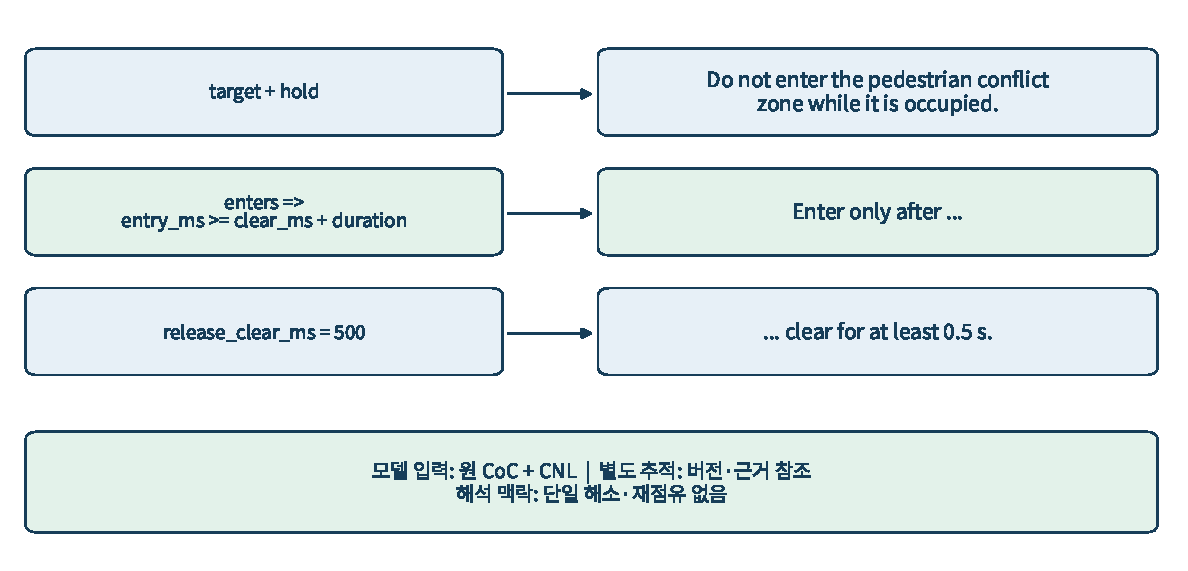
\includegraphics[width=\linewidth,height=.39\textheight,keepaspectratio]{figures/cnl-map-ko.pdf}
\par\small\raggedright 그림 5. 대상과 제한은 첫 문장에, 해제 기간과 포함 경계는 두 번째 문장에 대응한다. 원 CoC와 CNL은 함께 모델 입력에 들어가고 출처·버전은 추적 정보로 별도 보존한다. 색은 필드 대응을 구분하기 위한 것이며 추가 검증 수준을 뜻하지 않는다.
\end{minipage}\par\medskip

\subsection*{2. 의미 대응의 범위}

생성 단계에서는 대상, 부정, 조건의 방향, 시간값과 단위의 대응을 유지한다. 예를 들어 ‘최소 0.5초’에서 ‘최소’를 생략하거나 ‘이후에만 진입’을 ‘이후 반드시 진입’으로 바꾸면 허용 행동의 의미가 달라진다. 고정된 필드 대응은 이러한 변화를 명시적으로 확인할 수 있게 한다.\par

계약의 모든 메타데이터를 모델 입력 문장에 넣는 것은 아니다. 버전과 근거 참조는 데이터의 추적 정보로 유지하고, 행동 선택에 필요한 조건을 CNL에 표현한다. 모델링 가정은 실험 환경과 과제 정의에 명시한다. 따라서 이 문장과 JSON의 모든 필드가 문자 그대로 일대일 대응한다는 주장이 아니라, 지정한 맥락에서 행동 제한의 의미를 대응시킨다는 주장이다. 자유롭게 다시 작성한 문장이나 다른 프로파일로 확장할 때는 별도의 의미 검토가 필요하다.\par

\subsection*{3. CoC와 학습 입력의 결합}

원래 CoC는 행동 이유를 제공하고, 생성된 CNL은 추가적인 행동 조건을 제공한다. 두 텍스트를 결합하되 원문 CoC를 명세로 대체하지 않는다. 시간 예제에서 보강된 텍스트는 다음과 같다.\par

\begin{quote}Yield to the crossing pedestrian, then proceed through the intersection. Do not enter the pedestrian conflict zone while it is occupied. Enter only after the zone has remained clear for at least 0.5 s.\end{quote}

여기에 영상과 행동 후보를 함께 제시하고, 별도 참조 계산으로 정한 행동 라벨을 학습 목표로 둔다. P0에는 원 CoC, P1에는 원 CoC와 기존 자연어 제약, P2에는 원 CoC와 EBLC 기반 CNL을 제공한다. P1과 P2는 모두 제약을 추가한 접근이고, 주 비교는 CoC 단독 P0에 대한 제약 제공의 효과이다. EBLC 원문 JSON이나 솔버의 판정 결과를 정답 힌트로 입력하지 않는다.\par

주 실험의 P1·P2는 학습과 평가 모두에서 제약 문장을 제공한다. 그러므로 이 입력 구성은 명시된 규칙을 이용한 행동 선택을 평가하며, 평가 때 제약이 없어도 같은 규칙을 적용하는지를 직접 보여 주는 구성은 아니다. 특히 주 예제에서 P0에는 대기기간이 없으므로 두 계약이 다른 참조 행동을 요구해도 P0의 입력은 같을 수 있다. 이 정보 차이는 비교 조건의 일부로 공개한다.\par

추적 가능한 데이터 레코드에는 영상 참조, 원 CoC, 계약과 근거, CNL, 후보, 참조 행동 및 데이터 분할을 함께 기록하되, 모델에 제공할 필드와 정답·검증용 필드를 분리한다. 이에 따라 어떤 제약을 어떤 근거로 명세하고, 어떤 문장으로 전달하며, 어떤 행동을 학습 목표로 사용했는지 재구성할 수 있다. 구체적 학습 예산과 평가 지표는 다음 실험 절에서 제시한다.\par

\begingroup\small\setlength{\parskip}{3pt}
\subsection*{구현 및 예제 근거}

이 목록은 원고 검토를 위한 재현 근거이며, 외부 선행연구 인용과 구별한다. 전체 원고 통합 시 코드·데이터 공개 정보와 보충자료에 연결한다.\par

\begin{itemize}\setlength{\itemsep}{0pt}\setlength{\parsep}{0pt}\setlength{\topsep}{2pt}
\item \href{\detokenize{../../../../../../projects/04-guardsynth-coc/experiments/paper1_cnl_learning/temporal_preservation.py}}{S1 시간 계약·Core 변환·검증·CNL 생성}
\item \href{\detokenize{../../../../../../platforms/eblc-bcv/src/guard_synth_eblc/action_contract.py}}{S2 정성적 계약의 파서와 수명주기 의미}
\item \href{\detokenize{../../../../../../projects/04-guardsynth-coc/experiments/paper1_cnl_learning/temporal_training_data.py}}{S3 학습 입력과 독립 참조 계산}
\item \href{\detokenize{../../../../../../projects/04-guardsynth-coc/src/guard_synth/qualitative_scene_contract.py}}{S4 제한된 실제 장면 adapter}
\item \href{\detokenize{../methodology-2026-09-30-001/manuscript_examples.json}}{S5 원고 예제의 실행 질의와 결과}
\item \href{\detokenize{../methodology-2026-09-30-001/learning_input_examples.json}}{원고 예제의 두 학습 입력 레코드}
\end{itemize}
\endgroup
\end{document}